%% Преамбула TeX-файла

% 1. Стиль и язык
\documentclass[utf8x]{G7-32} % Стиль (по умолчанию будет 14pt)
\usepackage[T2A]{fontenc}
\usepackage[russian]{babel}
% Остальные стандартные настройки убраны в preamble.inc.tex.
\sloppy

% Настройки стиля ГОСТ 7-32
% Для начала определяем, хотим мы или нет, чтобы рисунки и таблицы нумеровались в пределах раздела, или нам нужна сквозная нумерация.
\EqInChapter % формулы будут нумероваться в пределах раздела
\TableInChapter % таблицы будут нумероваться в пределах раздела
\PicInChapter % рисунки будут нумероваться в пределах раздела

% Добавляем гипертекстовое оглавление в PDF
\usepackage[
bookmarks=true, colorlinks=true, unicode=true,
urlcolor=black,linkcolor=black, anchorcolor=black,
citecolor=black, menucolor=black, filecolor=black,
]{hyperref}

% Изменение начертания шрифта --- после чего выглядит таймсоподобно.
% apt-get install scalable-cyrfonts-tex

\IfFileExists{cyrtimes.sty}
    {
        \usepackage{cyrtimespatched}
    }
    {
        % А если Times нету, то будет CM...
    }

\usepackage{graphicx}   % Пакет для включения рисунков

% С такими оно полями оно работает по-умолчанию:
% \RequirePackage[left=20mm,right=10mm,top=20mm,bottom=20mm,headsep=0pt]{geometry}
% Если вас тошнит от поля в 10мм --- увеличивайте до 20-ти, ну и про переплёт не забывайте:
\geometry{right=20mm}
\geometry{left=30mm}


% Пакет Tikz
\usepackage{tikz}
\usetikzlibrary{arrows,positioning,shadows}

% Произвольная нумерация списков.
\usepackage{enumerate}

% ячейки в несколько строчек
\usepackage{multirow}

% itemize внутри tabular
\usepackage{paralist,array}


% Настройки листингов.
% 8 Листинги

\usepackage{listings}

% Значения по умолчанию
\lstset{
  basicstyle= \footnotesize,
  breakatwhitespace=true,% разрыв строк только на whitespacce
  breaklines=true,       % переносить длинные строки
%   captionpos=b,          % подписи снизу -- вроде не надо
  inputencoding=koi8-r,
  numbers=left,          % нумерация слева
  numberstyle=\footnotesize,
  showspaces=false,      % показывать пробелы подчеркиваниями -- идиотизм 70-х годов
  showstringspaces=false,
  showtabs=false,        % и табы тоже
  stepnumber=1,
  tabsize=4,              % кому нужны табы по 8 символов?
  frame=single
}

% Стиль для псевдокода: строчки обычно короткие, поэтому размер шрифта побольше
\lstdefinestyle{pseudocode}{
  basicstyle=\small,
  keywordstyle=\color{black}\bfseries\underbar,
  language=Pseudocode,
  numberstyle=\footnotesize,
  commentstyle=\footnotesize\it
}

% Стиль для обычного кода: маленький шрифт
\lstdefinestyle{realcode}{
  basicstyle=\scriptsize,
  numberstyle=\footnotesize
}

% Стиль для коротких кусков обычного кода: средний шрифт
\lstdefinestyle{simplecode}{
  basicstyle=\footnotesize,
  numberstyle=\footnotesize
}

% Стиль для BNF
\lstdefinestyle{grammar}{
  basicstyle=\footnotesize,
  numberstyle=\footnotesize,
  stringstyle=\bfseries\ttfamily,
  language=BNF
}

% Определим свой язык для написания псевдокодов на основе Python
\lstdefinelanguage[]{Pseudocode}[]{Python}{
  morekeywords={each,empty,wait,do},% ключевые слова добавлять сюда
  morecomment=[s]{\{}{\}},% комменты {а-ля Pascal} смотрятся нагляднее
  literate=% а сюда добавлять операторы, которые хотите отображать как мат. символы
    {->}{\ensuremath{$\rightarrow$}~}2%
    {<-}{\ensuremath{$\leftarrow$}~}2%
    {:=}{\ensuremath{$\leftarrow$}~}2%
    {<--}{\ensuremath{$\Longleftarrow$}~}2%
}[keywords,comments]

% Свой язык для задания грамматик в BNF
\lstdefinelanguage[]{BNF}[]{}{
  morekeywords={},
  morecomment=[s]{@}{@},
  morestring=[b]",%
  literate=%
    {->}{\ensuremath{$\rightarrow$}~}2%
    {*}{\ensuremath{$^*$}~}2%
    {+}{\ensuremath{$^+$}~}2%
    {|}{\ensuremath{$|$}~}2%
}[keywords,comments,strings]

% Подписи к листингам на русском языке.
\renewcommand\lstlistingname{\cyr\CYRL\cyri\cyrs\cyrt\cyri\cyrn\cyrg}
\renewcommand\lstlistlistingname{\cyr\CYRL\cyri\cyrs\cyrt\cyri\cyrn\cyrg\cyri}


% Полезные макросы листингов.
% Любимые команды
\newcommand{\Code}[1]{\textbf{#1}}

\newcommand{\myImage}[3]{
\begin{figure}[!ht]
    \centering
    \includegraphics[width=\textwidth]{figures/#2}
    \caption{#1}
    \label{#3}
\end{figure}
}


\begin{document}

\frontmatter % выключает нумерацию ВСЕГО; здесь начинаются ненумерованные главы: реферат, введение, глоссарий, сокращения и прочее.

% Команды \breakingbeforechapters и \nonbreakingbeforechapters
% управляют разрывом страницы перед главами.
% По-умолчанию страница разрывается.

% \nobreakingbeforechapters
% \breakingbeforechapters

\begin{abstract}

Работа описывает исследование параметризованной нелинейной системы
на наличие предельных циклов. В ходе исследования системы,
рассматриваются следующие вопросы: нахождение параметра системы, при котором 
наблюдается предельный цикл; поиск параметра, где наблюдается бифуркация поведения системы;
исследование свойств обнаруженного предельного цикла и определение характера его
устойчивости. Данные задачи изучаются путем проведения численных экспериментов
с помощью интерпретатора Python 3.5 и математических библиотек (numpy\cite{numpy},
matplotlib\cite{matplotlib}).

\end{abstract}

%%% Local Variables: 
%%% mode: latex
%%% TeX-master: "rpz"
%%% End: 


\tableofcontents

\mainmatter % это включает нумерацию глав и секций в документе ниже

\chapter{Поиск предельного цикла}

Рассмотрим исследуемую систему (уравнение \eqref{lab:eq:1},
$\nu$ - параметр системы). Она описывается
уравнением от одной фазовой переменной $x$. Уравнение дифференциальное, второго
порядка и, в силу слагаемого $3\dot{x}^3$, нелинейное. Решение такого уравнения
аналитическими методами является довольно сложной задачей, поэтому нашим
методом исследования будет построение численных экспериментов, описывающих
данную систему при определенном параметре $\nu$.

\begin{equation}\label{lab:eq:1}
  \ddot{x} + 3 \dot{x}^3 - \nu\dot{x} + x = 0
\end{equation}

Однако, в таком виде уравнение \eqref{lab:eq:1} не является удобным для
моделирования. Поэтому приведем его к канонической форме от двух переменных, с
помощью замены \eqref{lab:eq:2}, получив уравнение от двух фазовых переменных
$y_1$ и $y_2$ (Система уравнений \eqref{lab:eq:3}). В дальнейшем, мы будем
пользоваться описанием нашей системы именно в таком виде.

\begin{equation}\label{lab:eq:2}
  \begin{cases}
    &y_1 = x \\
    &y_2 = \dot{x}
  \end{cases}
\end{equation}

\begin{equation}\label{lab:eq:3}
  \begin{cases}
    &\dot{y_1} = y_2 \\
    &\dot{y_2} = -3y_2^3\ + \nu y_2 - y_1
  \end{cases}
\end{equation}

Преобразовав систему к удобному для нас виду, перейдем к первой части работы --
нахождения такого параметра $\nu$, при котором наблюдается предельный цикл.

Для начала, дадим определение искомому объекту.

\begin{definition}\label{lab:def:cycle}
  Предельным циклом будем называть замкнутую изолированную траекторию
  в фазовом пространстве, подразумевая замкнутость в смысле периодичности
  поведения системы.
\end{definition}

Таким образом, нам нужно построить фазовый портрет нашей системы, на котором
нужно будет обнаружить искомую замкнутую линию. Для этого, зная зависимость
значения производных от их координат, можно с помощью функции
\textit{streamplot}\cite{streamplot} построить фазовый портрет (Программа
\ref{lab1:prog:1}, в качестве параметра для начала возьмем $\nu = 1$).

\begin{program}
  \caption{Построение фазового портрета}
  \label{lab1:prog:1}
  \begin{verbatim}
# Подключение используемых библиотек
# В дальнейшем является постоянным и опускается в листингах
# Полный исходный код программы можно найти в приложении
import matplotlib.pyplot as plt
import numpy as np

# Параметр системы
nu = 1

# создание сетки 100х100 точек в области [-3;3]x[-3;3]
Y, X = np.mgrid[-3:3:100j, -3:3:100j]

# вычисление фазовых векторов на сетке
Y1 = Y
Y2 = -3 * Y ** 3 + nu * Y - X

# построение фазового портрета
fig0, ax0 = plt.subplots()
plt.streamplot(X, Y, Y1, Y2)

# показать построенные графики (опускается в дальнейшем)
plt.show()
  \end{verbatim}
\end{program}
\clearpage


\begin{figure}[thp]
  \centering
  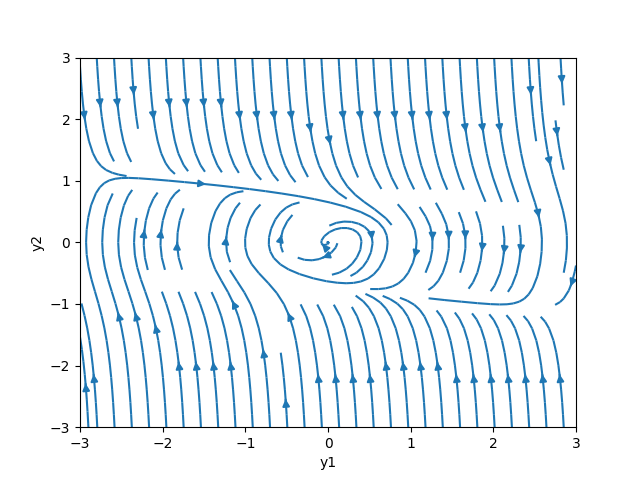
\includegraphics[width=\textwidth]{figures/1_streamplot}
  \caption{Поиск предельного цикла построением фазового портрета}
  \label{lab1:streamplot}
\end{figure}

На графике \ref{lab1:streamplot} изображен результат работы нашей программы.
В данном случае значение параметра оказалось оптимальным: можно видеть, как
изоклины сходятся к наклоненному прямоугольнику в центре графика.

Теперь, чтобы убедится наверняка, что траектории сходятся вокруг этого цикла
и там нет разрывов, построим две линии методом Эйлера снаружи и внутри наблюдаемого
цикла (Программа \ref{lab1:prog:2}).

\begin{program}
  \caption{Использование метода Эйлера для проверки предельного цикла}
  \label{lab1:prog:2}
  \begin{verbatim}
# функция построение кривой методом Эйлера
def line(y1_0, y2_0):
    y1 = [y1_0]
    y2 = [y2_0]
    h = 0.01 # длина шага
    for i in range(2000): # 2000 - количество итераций
        y1.append(y1[i] + h*(y2[i]))
        y2.append(y2[i] + h*(-3*y2[i] ** 3 + nu*y2[i] - y1[i]))
    # отображение кривой на графике
    ax0.plot(y1, y2)

# построение двух кривых, начинающихся внутри и
# вне предполагаемого предельного цикла
line(0.1, 0.1)
line(2, 2)
  \end{verbatim}
\end{program}

\clearpage

\begin{figure}[thp]
  \centering
  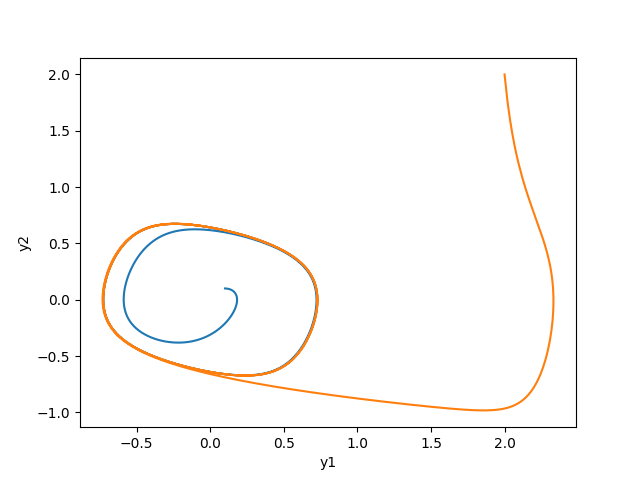
\includegraphics[width=\textwidth]{figures/1_cycle}
  \caption{Обнаружение аттрактора методом Эйлера}
  \label{lab1:cycle}
\end{figure}

На рисунке \ref{lab1:cycle} мы можем видеть две линии, начинающиеся из точек
$(0.1, 0.1)$ и $(2, 2)$. Эти линии сходятся сближаются к искомому предельному
циклу системы.

\chapter{Поиск точек бифуркаций}

Найдя предельный цикл в системе \eqref{lab:eq:3}, мы можем перейти к следующему
этапу нашего исследования -- определения всех значений параметра, при которых
наблюдается данный цикл.

В силу того, что наша система рассматривается дифференциальным уравнением,
поведение системы будет меняться плавно на промежутках, разделенных так
называемыми точками \textit{бифуркации}(точки, в которых происходит изменение
поведения системы).

\begin{definition}
    Точка бифуркации - значение параметра системы, при котором наблюдается
    качественное изменение поведения системы.
\end{definition}

Чтобы нам было удобно наблюдать изменение системы от параметра без перезапуска
программы, мы обернем построения в функцию и добавим в нашу программу слайдер --
бегунок, которым можно будет менять значение параметра $\nu$.

\begin{figure}
    \centering
    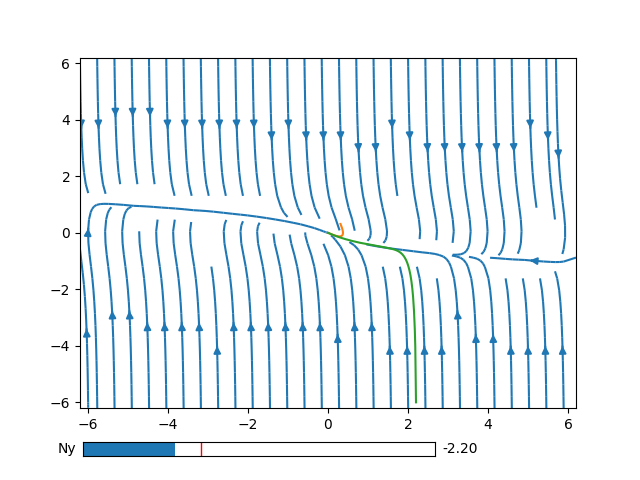
\includegraphics[width=0.8\textwidth]{figures/2_point_-2_2}
    \caption{Стационарная точка системы при $\nu = -2.2$}
    \label{lab2:point_-2}
\end{figure}

Начиная с отрицательных значений (от -10) мы наблюдаем сильное стремление
к центру координат -- стационарной точки системы (График \ref{lab2:point_-2}).

\begin{figure}[!ht]
    \centering
    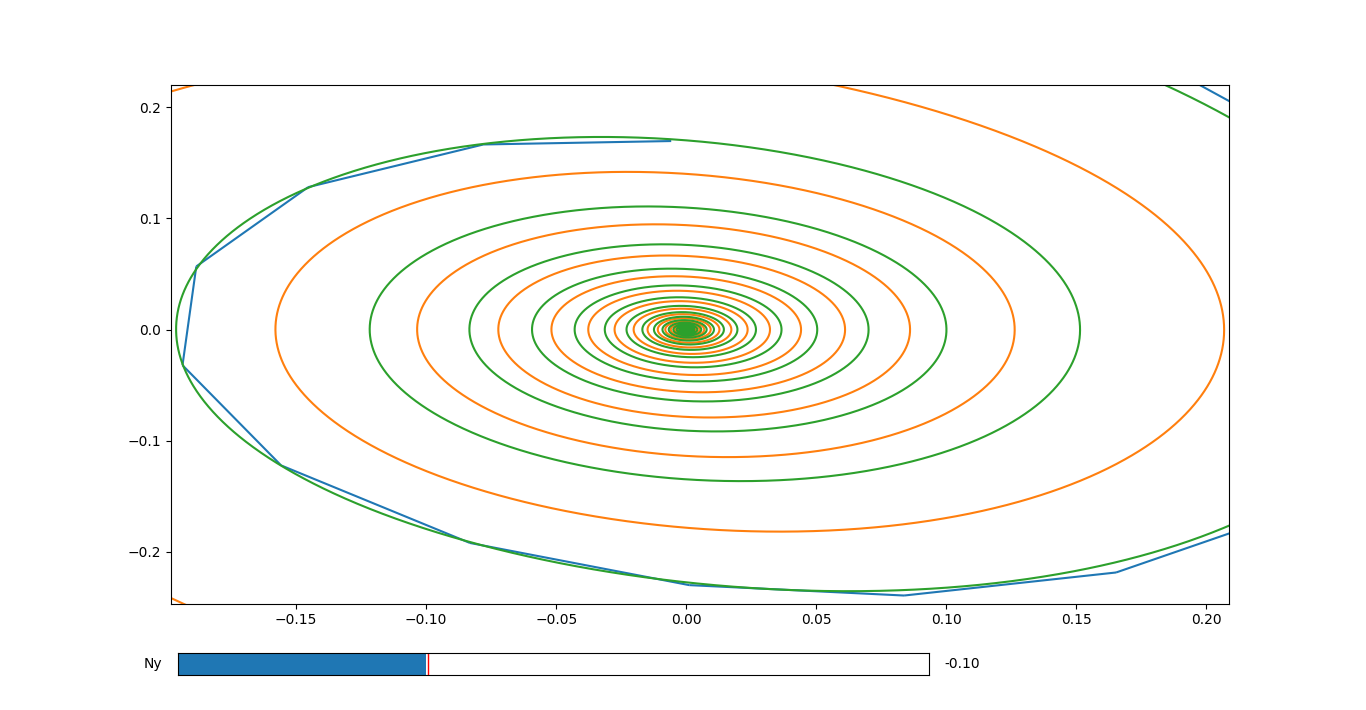
\includegraphics[width=0.8\textwidth]{figures/2_point_-0_1}
    \caption{Стационарная точка системы при $\nu = -0.1$}
    \label{lab2:point_0}
\end{figure}

При приближении параметра к нулю, поведение системы искривляется в овальную
форму, но линии медленно сходятся к нулю (График \ref{lab2:point_0}).

\begin{figure}[!ht]
    \centering
    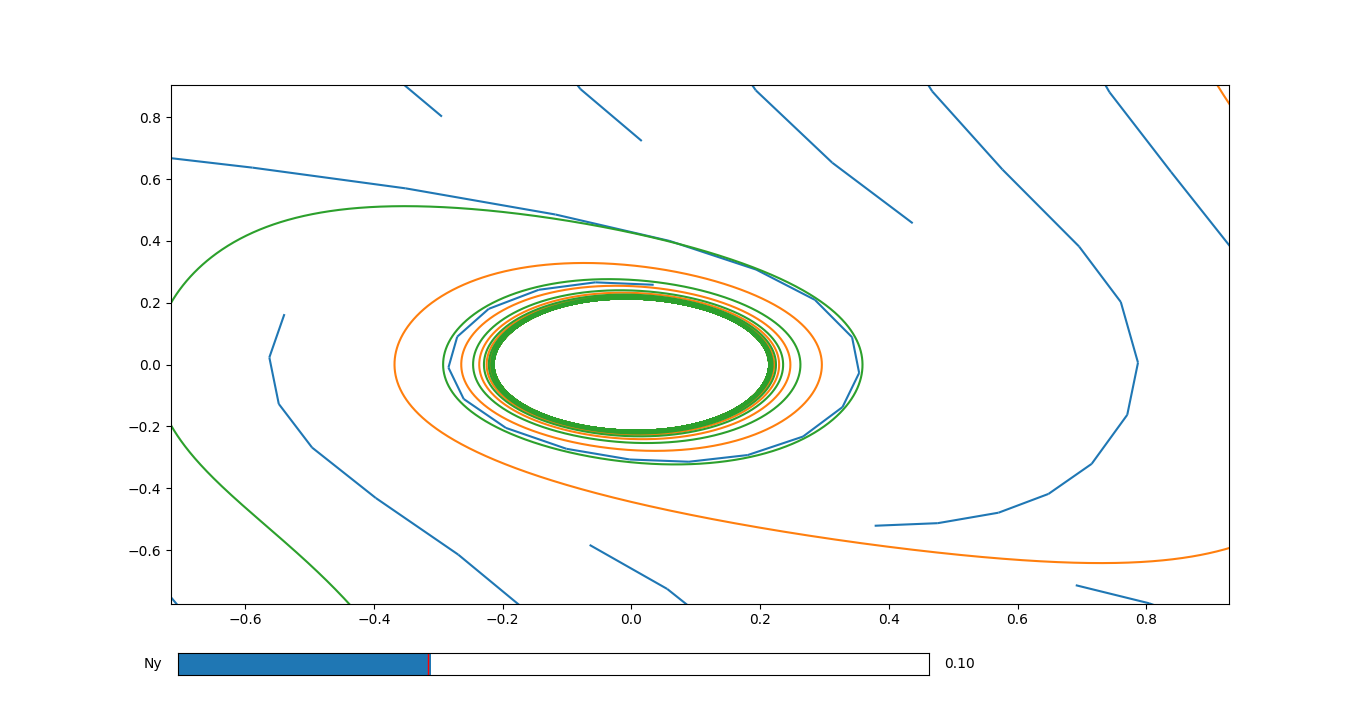
\includegraphics[width=0.8\textwidth]{figures/2_cycle_0_1}
    \caption{Появление цикла при $\nu = 0.1$}
    \label{lab2:cycle_0_1}
\end{figure}

Как только мы переступаем нулевое значение параметра, наши траектории
останавливаются значительно раньше -- мы начинаем наблюдать знакомый нам
предельный цикл, но в меньших размерах (График \ref{lab2:cycle_0_1}).

\begin{figure}[!ht]
    \centering
    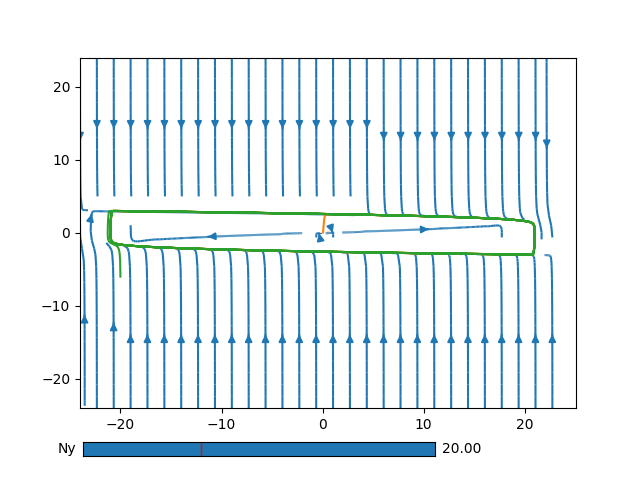
\includegraphics[width=0.8\textwidth]{figures/2_cycle_20}
    \caption{Расширение предельного цикла при увеличении параметра ($\nu = 20$)}
    \label{lab2:cycle_20}
\end{figure}

Увеличивая $\nu$ дальше, остается наблюдать за ростом цикла (График
\ref{lab2:cycle_20}).

Из полученных наблюдений можно выдвинуть гипотезу: на отрицательной полуоси
исследуемая система сходится в стационарную точку; в положительной же оси
наблюдается предельный цикл, который увеличивается в зависимости от параметра
системы.

Стоит отметить, что наличие или отсутствие предельного цикла на границе
($\nu = 0$) мы выявить не можем, так как при приближении к параметра к нулю,
чтобы быть уверенным в наличии стационарной точки или цикла, приходится
увеличивать точность вычислений. В конце концов, когда точность увеличить
не удается, нам остается только предполагать: толи линии сошлись к циклу, толи
они не достигли нуля из-за недостаточного кол-ва шагов в методе Эйлера.

С учетом этого замечания, можно выдвинуть еще одну гипотезу: так как изменение
поведения в системе происходит настолько плавно, что нам не удается уловить
момент, когда мы наблюдаем стационарную точку, а когда предельный цикл.
То есть мы можем говорить, что наблюдается \textit{мягкая бифуркация системы}.

\chapter{Исследование свойств предельного цикла}

Следующим шагом в исследовании системы станет изучение свойств нашего
предельного цикла при конкретном значении параметра (возьмем $\nu = 1$):
нахождение его периода (от независимой переменной) и его форму. Данные свойства
потребуются в следующих частях (\ref{lab4} и \ref{lab5}) для проверки
характера его устойчивости.

Ставя численные эксперименты, значения могут получатся точные, но все же с
погрешностью. Поэтому далее мы будем находить значение с точностью до 3-х знаков
после запятой (т. е. наше значение должно расходится не более чем на
$\epsilon = 0.5 * 10 ^{-4}$).

В программе \ref{lab3:prog:1} строится цикл методом точечных отображений Пуанкаре:
выбирается точка на оси $0_{y1}$, от которой мы начинаем двигаться по траектории
до тех пор, пока снова не пересечет ось. При приближении к нашему предельному
циклу, точки будут сближаться все больше и больше. Таким образом будем считать
траекторию предельным циклом, когда начальная и конечная точка сблизятся по
обоим координатам ближе чем на $\epsilon$. Периодом нашего цикла будет
количество затраченных шагов ($i + 1$) помноженных на длину шага $h$.
Как видно из работы программы, цикл имеет период $\omega = 6.663$.

Далее можно попытаться найти аналитическую форму данного цикла, но судя по
графику \ref{lab1:cycle} форма цикла не похожа на знакомые квадратичные функции и
подбор аналитического вида кривой может оказаться трудной задачей. При этом мы
не сможем достигнуть такой же точности, как наше поточечное решение, полученное
методом Эйлера. Поэтому в следующих работах будем работать с массивами $y1$ и
$y2$, описывающие наш цикл.

\begin{program}
    \caption{Поиск параметров системы}
    \label{lab3:prog:1}
    \begin{verbatim}
eps = 0.5 * 10 ** -4
y1_0, y2_0 = 0.72424, 0 # начальная точка

y1 = [y1_0]
y2 = [y2_0]
h = 0.0001
for i in range(100000):
    # итерация метода Эйлера
    y1.append(y1[i] + h*(y2[i]))
    y2.append(y2[i] + h*(-3*y2[i] ** 3 + ny * y2[i] - y1[i]))
    # проверка прихода в туже точку с погрешностью
    if  np.abs(y1_0 - y1[i+1]) < eps and
        np.abs(y2_0 - y2[i+1]) < eps:
        # вывод результатов
        print("h={h}, i={i}, h*i={period}".format(
              h=h, i=i+1, period=h*(i+1)))
        return;
# Вывод программы
# h=0.0001, i=66633, h*i=6.6633000000000004
    \end{verbatim}
\end{program}




\backmatter %% Здесь заканчивается нумерованная часть документа и начинаются ссылки и
            %% заключение

\Conclusion % заключение к отчёту

В результате проделанной работы стало ясно, что ничего не ясно...

%%% Local Variables: 
%%% mode: latex
%%% TeX-master: "rpz"
%%% End: 


% % Список литературы при помощи BibTeX
% Юзать так:
%
% pdflatex rpz
% bibtex rpz
% pdflatex rpz

\bibliographystyle{gost780u}
\bibliography{rpz}

%%% Local Variables: 
%%% mode: latex
%%% TeX-master: "rpz"
%%% End: 


\appendix   % Тут идут приложения

\chapter{Исходный код}
\label{appendix:src}

\begin{program}
  \caption{Поиск предельного цикла - построение фазового партрета}
  \begin{verbatim}
import matplotlib.pyplot as plt
import numpy as np
# создание сетки 100х100 точек в области [-3;3]x[-3;3]
Y, X = np.mgrid[-3:3:100j, -3:3:100j]

# Параметр системы
nu = 1
# вычисление фазовых векторов на сетке
Y1 = Y
Y2 = -3 * Y ** 3 + nu * Y - X

# построение фазового портрета
fig0, ax0 = plt.subplots()
plt.streamplot(X, Y, Y1, Y2)

# подпись осей на графике
ax0.set_xlabel("y1")
ax0.set_ylabel("y2")
# показать построенные графики
plt.show()
  \end{verbatim}
\end{program}

\begin{program}
  \caption{Поиск предельного цикла - обнаружение предельного цикла методом Эйлера}
  \begin{verbatim}
import matplotlib.pyplot as plt
import numpy as np

fig0, ax0 = plt.subplots()
# подпись осей на графике
ax0.set_xlabel("y1")
ax0.set_ylabel("y2")

# Параметр системы
nu = 1
# функция построение кривой методом Эйлера
def line(y1_0, y2_0):
    y1 = [y1_0]
    y2 = [y2_0]
    h = 0.01 # длина шага
    for i in range(2000): # 200o - количество итераций
        y1.append(y1[-1] + h*(y2[-1]))
        y2.append(y2[-1] + h*(-3*y2[-1] ** 3 + nu*y2[-1] - y1[-1]))
    # отображение кривой на графике
    ax0.plot(y1, y2)

# построение двух кривых, начинающихся внутри и 
# вне предпологаемого предельного цикла
line(0.1, 0.1)
line(2, 2)
# показать построенные графики
plt.show()
  \end{verbatim}
\end{program}
%%% Local Variables: 
%%% mode: latex
%%% TeX-master: "rpz"
%%% End: 

\chapter{Еще картинки}
\label{cha:appendix2}

\begin{figure}
\centering
\caption{Еще одна картинка, ничем не лучше предыдущей. Но надо же как-то заполнить место.}
\end{figure}

%%% Local Variables: 
%%% mode: latex
%%% TeX-master: "rpz"
%%% End: 


\end{document}

%%% Local Variables:
%%% mode: latex
%%% TeX-master: t
%%% End:
